\setcounter{section}{1}
\section*{Annexe A}
\label{annexe:A}
\addcontentsline{toc}{section}{Annexe A}

\subsection{Fonctionnement détaillé des solutions de \gls{pam}}

Nous détaillerons dans cette annexe, le fonctionnement détaillé d'une solution de \gls{pam}. Afin d'illustrer les propos tenus, nous nous appuierons sur des schémas et digrammes de séquences.\\
Avant d'expliquer le fonctionnement d'une solution de \gls{pam}, nous allons voir comment les systèmes fonctionnent en temps normal.

\subsubsection{Sans solution de \gls{pam}}
\label{par:nopam}

Dans ce scénario, les utilisateurs finaux possèdent le mot de passe d'accès direct à la ressource protégée, comme on peut le voir sur la \textsc{Figure} \ref{fig:sans_PAM}.

\begin{figure}[!ht]
    \center
    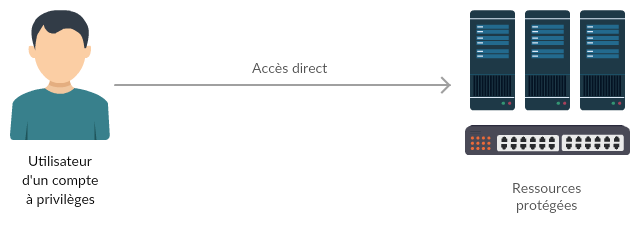
\includegraphics[width=\textwidth]{./images/Schema_ultra_light_sans_PAM.png}
    \caption{Connexion à une ressource protégée sans solution de \gls{pam}}
    \label{fig:sans_PAM}
\end{figure}

On remarque qu'ici, les utilisateurs accèdent directement aux ressources protégées avec des mots de passe dédiés à chaque service/application/matériel. Il est donc très fréquent car inévitable que des utilisateurs partagent le même mot de passe. De plus, n'ayant aucune fédération (pas de supervision, ni de traçage), l'utilisateur est apte à effacer ses traces, par exemple en vidant les logs des applications et de ses actions\footnote{Par exemple sous Debian 8, la commande \texttt{cat /dev/null > ~/.bash\_history \&\& history -c \&\& exit} supprime toute action effectuée sur la machine avec le compte courant.}. On ne peut donc pas savoir ce que l'utilisateur a fait, ni quel utilisateur a fait des actions sur la ressource cible.\\
Le diagramme de séquence en \textsc{Figure} \ref{fig:diagseq_sans_PAM} décrit en détail les action qui se déroulent lors d'une telle connexion. Il permet de aussi de mettre en évidence l'absence de contrôle des utilisateurs : aucun registre d’événements ne prend en compte les actions des utilisateurs. Les utilisateurs se partageant le même mot de passe pour chaque ressource cible, le contrôle n'est ainsi plus mis sur les utilisateurs, mais sur les ressources cibles, ce qui est l'opposé de ce que nous cherchons à faire. La \textsc{Figure} \ref{fig:invcont} schématise cette inversion du contrôle. 

\begin{figure}[!ht]
    \center
    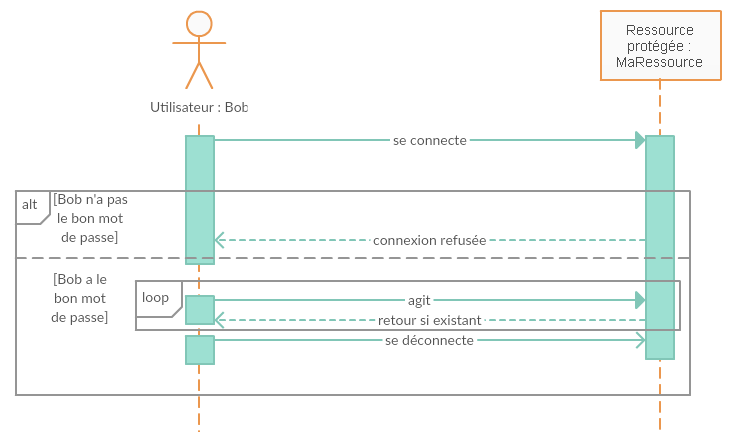
\includegraphics[width=\textwidth]{./images/Sequence_noPAM_use.png}
    \caption{Diagramme de séquence détaillant les actions effectuées lors d'une connexion à une ressource sans solution de \gls{pam}}
    \label{fig:diagseq_sans_PAM}
\end{figure}

\begin{figure}[!ht]
    \center
    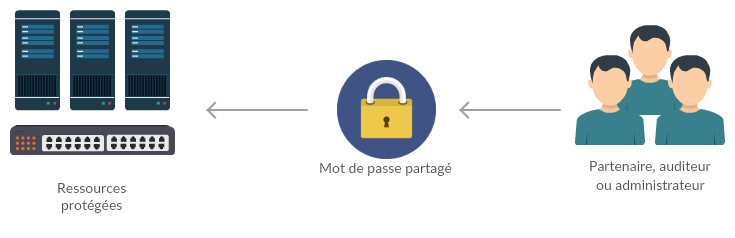
\includegraphics[width=\textwidth]{./images/ressource_centered.png}
    \caption{Schéma mettant en évidence l'inversion du contrôle de sécurité, mis sur les ressources plutôt que sur les utilisateurs}
    \label{fig:invcont}
\end{figure}

\subsubsection{Avec solution de \gls{pam}}
\label{par:withpam}

Dans ce scénario, une solution de \gls{pam} est en place. Ainsi les utilisateurs n'ont pas d'accès direct aux ressources cible. Toute l'architecture s'articule autour d'un composant central : le contrôleur d'accès appelé \gls{bastion}. Tout accès à une ressource cible se fait via ce \gls{bastion}. Cette architecture centralisée est schématisée dans la \textsc{Figure} \ref{fig:schempam}. Nous allons reprendre point par point un scénarion de connexion réussie à une ressource cible (en correspondance avec les étapes de la \textsc{Figure} \ref{fig:schempam}).

\begin{figure}[!ht]
    \center
    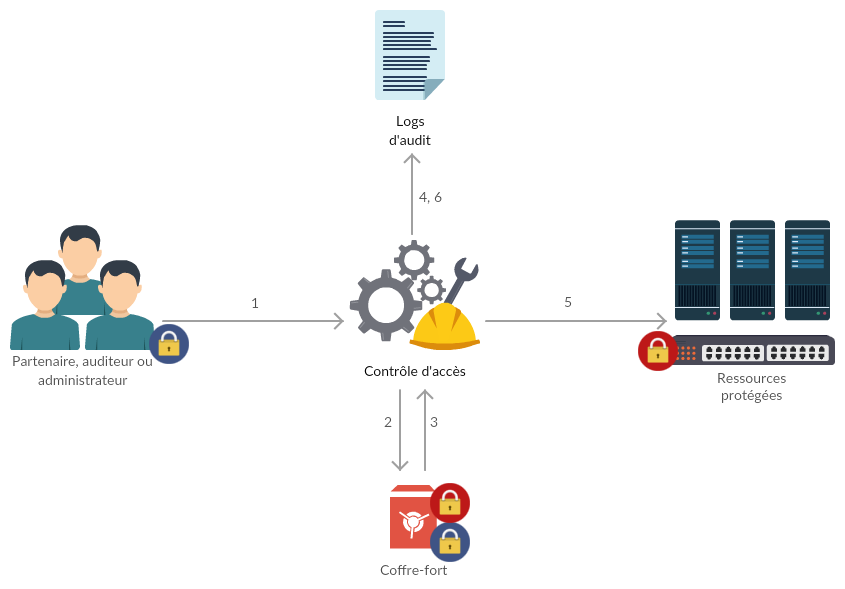
\includegraphics[width=\textwidth]{./images/Schema_PAM.png}
    \caption{Schéma décrivant l'architecture d'une solution de \gls{pam} intégrée dans une infrastructure}
    \label{fig:schempam}
\end{figure}

\begin{enumerate}
	\item L'utilisateur se connecte au \gls{bastion} avec ses \glspl{credential}, que l'on appellera ses accès primaires (cadenas bleu)
	\item Le \gls{bastion} vérifie l'identité de l'utilisateur en interrogeant le base de données du coffre-fort
	\item Le coffre-fort retourne un jeton, qu'on appellera accès secondaire (cadenas rouge), pour se connecter à la ressource cible si l'identification primaire est bonne
	\item Le \gls{bastion} génère des logs de connexion
	\item L'utilisateur se connecte à la ressource protégée via la \gls{bastion} qui lui fournit les accès secondaires
	\item Chaque action de l'utilisateur est logué par le \gls{bastion}, tout comportement interdit alerté voir coupe la connexion à la ressource
\end{enumerate}

Afin de détailler toutes les actions effectuées, nous allons décrire chaque étape, pour tous les cas d'utilisation, dans le diagramme de séquence en \textsc{Figure} \ref{fig:diagseq_PAM}.

\begin{figure}[!ht]
    \center
    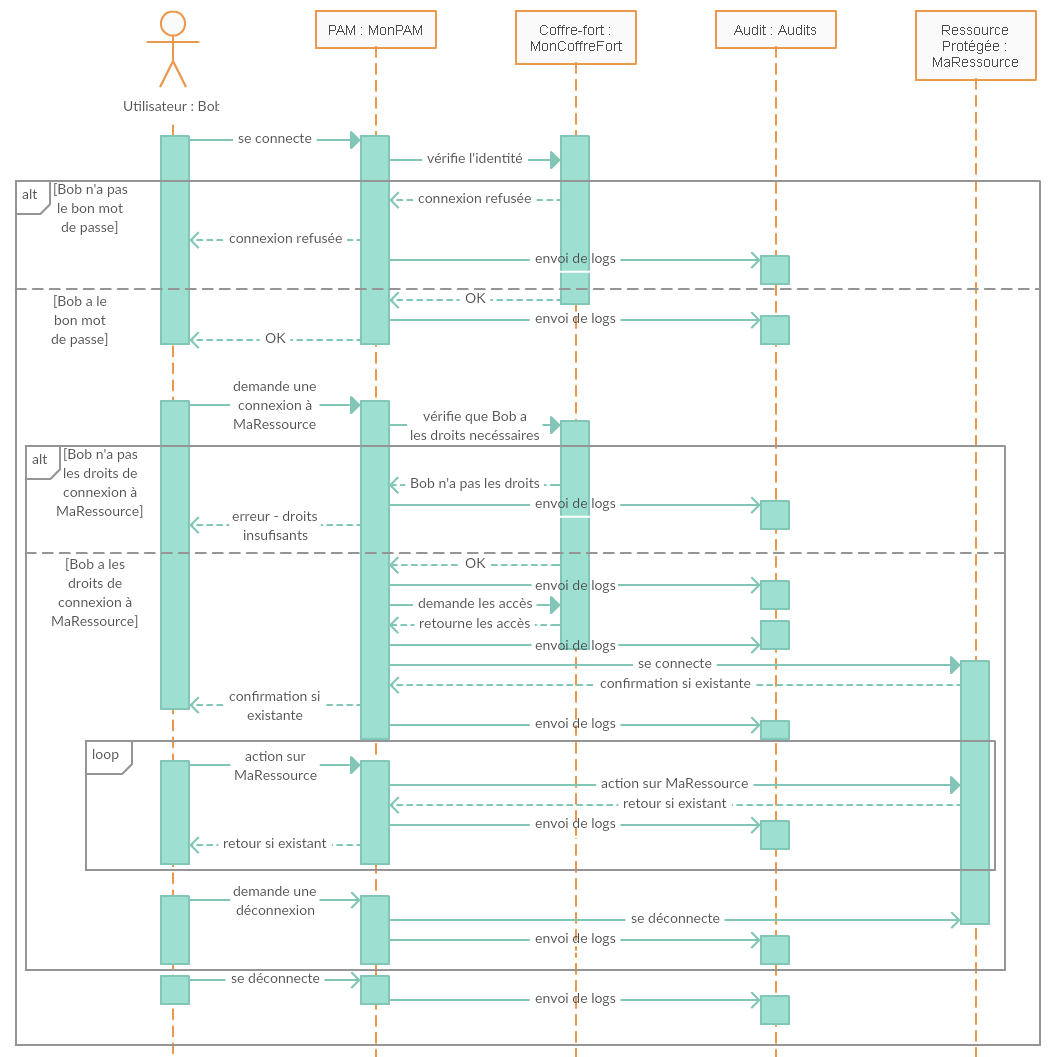
\includegraphics[width=1.2\textwidth]{./images/Sequence_PAM_use.png}
    \caption{Diagramme de séquence détaillant les actions effectuées lors d'une connexion à une ressource avec une solution de \gls{pam}}
    \label{fig:diagseq_PAM}
\end{figure}



Pour ne pas nous égarer dans les explications, les diagramme sera expliqué dans son fonctionnement intrinsèque.

\begin{itemize}
	\item Chaque ligne verticale représente un objet ou un utilisateur. Les utilisateurs sont représentés par un bonhomme, les objet par des cases
	\item Plus l'on descend sur ces lignes verticales, plus l'on avance dans le temps
	\item Les cadres représentent des boucles ou des conditions :
	\begin{arrowlist}
		\item \texttt{alt} : condition "si", la condition est explicitée en haut à gauche, les deux possibilités sont séparées par une ligne discontinue
		\item \texttt{loop} : boucle qui tourne de 0 à N fois, N étant un entier naturel
	\end{arrowlist}
	\item Chaque rectangle sur une ligne de temps (ligne verticale) représente une séquence d'actions
	\item Les flèches représentent des messages qui peuvent être :
	\begin{arrowlist}
		\item Asynchrones (n'attendent pas de retour) : flèches simples
		\item Synchrone (requête et réponse) : pour la requête, flèche simple avec le bout plein (triangle), pour la réponse, flèche en pointillés
	\end{arrowlist}
\end{itemize}

On peut alors voir 4 étapes :

\begin{enumerate}
	\item Une étape de connexion de l'utilisateur au \gls{bastion} avec ses accès primaires (qui aboutit ou pas selon la légitimité de l'utilisateur)
	\item Une étape de connexion de l'utilisateur à le ressource cible avec des accès secondaires fournis par le \gls{bastion} (via le coffre-fort)
	\item Une étape d'actions sur le ressource cible
	\item Une dernière étape de déconnexion
\end{enumerate}

Durant toute ces étapes, des logs sont envoyés par le \gls{bastion}, afin de conserver toutes les traces des actions effectuées par l'utilisateur. On peut alors clairement faire la différence avec la présence d'une solution de \gls{pam} :

\begin{itemize}
	\item Les utilisateurs sont suivis individuellement
	\item Chaque utilisateur est identifiable
	\item L'accès aux ressources cibles n'est pas direct, ce qui ajoute une couche de sécurité
	\item L'utilisateur utilisant un jeton (accès secondaire) pour se connecter aux ressources cibles, il n'a donc plus besoin de connaître ces mots de passe secondaires. Ils peuvent donc être changés périodiquement pour rendre la connexion sans solution de PAM impossible
\end{itemize}